\documentclass{../indiv}
\graphicspath{{../../images/part1/ch1/}}
\setcounter{chapter}{0}

\begin{document}
	\onlyifstandalone{\makebarother}
	\chapter{\LaTeX 簡介}
	歡迎各位讀者進入\LaTeX 的世界!在真正開始使用\LaTeX 前,先讓我們揭開\LaTeX 複雜的身世背景、看看\LaTeX 強大的威力吧!(怎麼寫得有點中二= =)
	
	\section{什麼是\TeX ?}
	\TeX 是美國電腦科學家Donald Knuth最初在1978年發表的一套排版軟體,同時也是一種標記式語言(Markup Language)。相較於市面上大多的排版軟體(如: Microsoft Word、LibreOffice Writer、Google Docs),\TeX 沒有漂亮的圖形化介面(GUI),而是像寫程式一樣,先把指令(告訴電腦文字與版面應該長怎樣)與文件內容(真的給人看的東西)寫在一個純文字檔後,再經過編譯器(Compiler)的編譯,產生最後可供人類閱讀的文件檔。
	
	\begin{extra}
		\item 為了與\TeX 後續衍生出的一大堆程式區別,這種最早出現、最陽春的\TeX 也經常被稱為原版\TeX (Plain \TeX)。
	\end{extra}
	
	\section{什麼是\LaTeX ?}
	隨著科技的發展,當年的原版\TeX 所提供的功能早已不敷使用,同時也被人覺得太複雜、不親民。因此,美國又有一位電腦科學家Leslie Lamport在1984年發表了基於\TeX 的排版系統\LaTeX ,支援更多實用的功能和更親民的指令集,也推廣了這整套系統的應用。 
	
	講白話一點,\LaTeX 其實就是\TeX 的PRO版,而且比原本的\TeX 好用n百倍,導致\TeX 已經被大眾打入冷宮了。
	
	\begin{figure}[H]
		\centering
		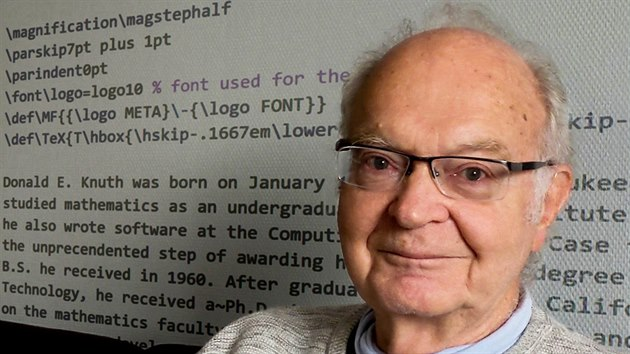
\includegraphics[height=4cm]{Donald_Knuth.jpg}
		\hspace{2mm}
		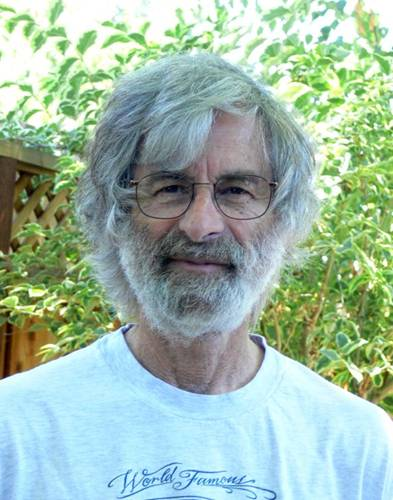
\includegraphics[height=4cm]{Leslie_Lamport.jpg}
		\caption{(左) Donald Knuth  (右) Leslie Lamport}
		\label{fig: Founders of TeX and LaTeX}
	\end{figure}
	
	\newpage
	\section{為什麼厲害的人都在用\LaTeX ?}
	\LaTeX 的功能非常強大、應用也十分廣泛,除了最主要被用於國際上的各大科學領域的文獻與教科書外,其實我們也可用\LaTeX 輕而易舉地做出精美的筆記、報告、履歷、甚至是投影片。以下是幾個\LaTeX 的特色與優點:
	\begin{itemize}
		\item \textbf{數學公式間距調整:}\LaTeX 幾乎就是為了排版數學公式而生的,其內部的演算法可配合當前字型,自動調整數學公式中數字與符號間的距離;使用者也可用指令手動增加或減少間距大小。
		\item \textbf{萬用的純文字檔案:}\LaTeX 的原始碼以純文字檔案儲存,因此檢視與編輯時不受作業系統或裝置限制,只要是打得出字的機器都能直接編輯。假設你的檔案是純英文,甚至可以用摩斯電碼傳給你朋友。
		\item \textbf{一勞永逸的格式設定:}一份LaTeX文件的所有格式設定都是透過指令達成的,因此格式設定只須寫一次,之後的新文件若要使用同樣的格式,就只要無厘頭的把整串格式設定的指令複製過去即可。網路上也有許多已經刻好的範本,可以直接下載下來使用。
		\item \textbf{穩定性:}一樣的原始碼即使在不同機器上編譯,理論上也會輸出一模一樣的檔案。不像Word或Google Docs,有時會出現同個檔案在另一台電腦上就莫名其妙格式跑掉或根本無法開啟的狀況。
		\item \textbf{完全免費:}所有\TeX 大家族的軟體都是完全免費的,當然也包括\LaTeX 與大部分的實用套件(Package)。
		\item \textbf{廣大的套件支援:}\LaTeX 目前可支援的套件高達6,000多個,幾乎可包辦所有你想得到的需求。裡面除了有方便管理參考文獻、製作圖表與投影片的工具外,其實也藏著許多令人意想不到的套件...。(詳見表~\ref{tab:Scientific Applications of LaTeX}與表~\ref{tab:Fun Applications of LaTeX})
		\item \textbf{神秘感:}讓你看起來很像某個資訊電神在寫程式;或是像某個駭客在入侵學校系統盜段考考卷出來,洩題給同學之後再跟他們討錢。
	\end{itemize}
	\vspace{0.1\baselineskip}
	\begin{figure}[H]
		\centering
		\mpimg{0.3}{arial-times-new-roman-i-use-latex-btw-46701863.png}
		\hspace{1cm}
		\mpimg{0.4}{s2uk3yloola21.jpg}
		\caption{兩張關於\LaTeX 的梗圖}
	\end{figure}
	
	\newpage
	\section{\LaTeX 究竟有多強大?}{%limit scope of "column type Z" and "setminted" to this section only
		\newcolumntype{Z}{Tp{4.5em}|>{\small\ttfamily}p{12ex}|>{\centering\arraybackslash\sffamily}p{5.05cm}|p{5.75cm}T}
		\setminted{fontsize=\tiny, breakafter=-=, breakbefore=\\, tabsize=2}
		
		說了這麼多,就讓我們實際看看\LaTeX 在數學公式與科學圖表優秀的排版能力吧!
		\begin{table}[H]
			\centering
			\rowcolors{2}{gray!20}{gray!10}
			\begin{tabular}{Z}
				\Thline
				\rowcolor{cyan!40} \thead{應用} & \thead{\textrm{套件}} & \thead{\textrm{範例}} & \thead{原始碼}(部分省略) \\ \hline
				數學公式 & amsmath &
				\begin{tabmp}
					\centering
					$ \displaystyle \hat{f}(\xi) = \int_{-\infty}^{\infty} f(x)\, e^{-2\pi ix\xi}\, dx $ 
				\end{tabmp} &
				\begin{tabmp}[-0.2]
					\begin{minted}{LaTeX}
\[ \hat{f}(\xi) = \int_{-\infty}^{\infty} f(x) e^{-2\pi ix\xi} dx \]
					\end{minted}
				\end{tabmp} \\ \hline
				化學\newline 結構式 & chemfig &
				\begin{tabmp}
					\centering
					\tabfig{\chemname[3.5ex]{\chemfig[angle increment=30]{*6(-=(--[1]-[-1]-[1]-[-1])-=(-OH)-(*6(-(<:[1]H)(*6(-=(-)---))-(<[7]H)-(-[6])(-[8])-O-))=)}}{\Large 四氫大麻酚(Tetrahydrocannabinol, THC)}}
				\end{tabmp} &
				\begin{tabmp}[-0.2]
					\begin{minted}{LaTeX}
\chemname[3ex]{\chemfig[angle increment=30]{
*6(-=(--[1]-[-1]-[1]-[-1])-=(-OH)-(*6(-(<:[1]H)
(*6(-=(-)---))-(<[7]H)-(-[6])(-[8])-O-))=)}
}{四氫大麻酚(Tetrahydrocannabinol, THC)}
					\end{minted}
				\end{tabmp} \\ \hline
				電路圖 & circuitikz &
				\begin{tabmp}
					\centering
					\tabfig{
						\begin{circuitikz}
							\fill[blue!15!white] (-1, 0.8) rectangle (0.5,-0.8);
							\fill[orange!20!white] (-1, -1.2) rectangle (0.5, -2.8);
							\node[draw, color=blue] at (1.7, 0){\textbf{P-channel}};
							\node[draw, color=orange] at (1.7, -2){\textbf{N-channel}};
							\ctikzset{tripoles/pmos style/emptycircle}						
							\draw (0,0) node[pmos](P){};
							\draw (0, -2) node[nmos](N){};
							\draw (P.D) -- (N.D);
							\draw (P.S) to[short, -*] ++(0, 0.5) node[above]{$V_{dd}$};
							\draw (N.S) -- ++(0, -0.5) node[ground](GND){}
							(GND.south) node[below]{$GND$};
							\draw (P.G) -- ++(-1, 0) -- ++(0, -1) node[](in){} -- ++(0, -1) -- (N.G);
							\draw (in.center) to[short, *-*] ++(-1, 0) node[left]{$V_{in}$};
							\draw (0, -1) to[short, *-*] ++(1, 0) node[right]{$V_{out}$};
						\end{circuitikz}
					}
				\end{tabmp} &
				\begin{tabmp}[-0.2]
					\begin{minted}{LaTeX}
\begin{circuitikz}
	% 繪製彩色方塊與文字標示
	\fill[blue!15!white] (-1, 0.8) rectangle (0.5,-0.8);
	\fill[orange!20!white] (-1, -1.2) rectangle (0.5, -2.8);
	\node[draw, color=blue] at (1.7, 0){\textbf{P-channel}};
	\node[draw, color=orange] at (1.7, -2){\textbf{N-channel}};
	% 繪製 PMOS 與 CMOS
	\draw (0,0) node[pmos](P){};
	\draw (0, -2) node[nmos](N){};
	% 繪製電線、接點與接點文字標示
	\draw (P.D) -- (N.D);
	\draw (P.S) to[short, -*] ++(0, 0.5) node[above]{$V_{dd}$};
	\draw (N.S) -- ++(0, -0.5) node[ground](GND){}
	(GND.south) node[below]{$GND$};
	\draw (P.G) -- ++(-1, 0) -- ++(0, -1) node[](in){} -- ++(0, -1) -- (N.G);
	\draw (in.center) to[short, *-*] ++(-1, 0) node[left]{$V_{in}$};
	\draw (0, -1) to[short, *-*] ++(1, 0) node[right]{$V_{out}$};
\end{circuitikz}
					\end{minted}
				\end{tabmp} \\ \Thline
			\end{tabular}
			\caption{\LaTeX 的科學應用範例}
			\label{tab:Scientific Applications of LaTeX}
		\end{table}
		\pagebreak
		但是這麼強大的軟體,不拿來做一些趣味應用真是太可惜了!其實\LaTeX 中也包含許多意想不到的套件,讓我們可以排版出科學用途之外的東西。以下是幾個有趣的例子:
		\begin{table}[H]
			\centering
			\rowcolors{2}{gray!20}{gray!10}
			\begin{tabular}{Z}
				\Thline 
				\rowcolor{cyan!40} \thead{應用} & \thead{\textrm{套件}} & \thead{\textrm{範例}} & \thead{原始碼}(部分省略) \\ \hline
				西洋棋 & skak \newline texmate &
				\begin{tabmp}
					\vspace{-0.8\baselineskip}
					\renewcommand{\afterno}{.}
					\whitename{Adolf Anderssen}
					\blackname{Jean Dufresne}
					\chessevent{Berlin/Berlin GER/1852}
					\chessopening{Evans Gambit}
					\ECO{C52}
					\tiny
					\makegametitle
					\begin{texmate}
						1.e4 e5 2.Nf3 Nc6 3.Bc4 Bc5 4.b4 Bxb4 5.c3 Ba5 6.d4 exd4 7.O-O d3 8.Qb3 Qf6 9.e5 Qg6 10.Re1 Nge7 11.Ba3 b5 12.Qxb5 Rb8 13.Qa4 Bb6 14.Nbd2 Bb7 15.Ne4 Qf5 16.Bxd3 Qh5 17.Nf6+ gxf6 18.exf6 Rg8 19.Rad1 Qxf3 20.Rxe7+ Nxe7 21.Qxd7+ Kxd7 22.Bf5+ Ke8 23.Bd7+ Kf8 24.Bxe7\# \result{1-0}
					\end{texmate}
					\vspace{2mm}
					\smallboard
					\notationon
					\preparediagram{Evergreen Game}{(Final position after 24.Bxe7\#)}
					\centering
					\tabfig[0.85]{\makediagrams}
				\end{tabmp} &
				\begin{tabmp}[-0.2]
					\begin{minted}{LaTeX}
% 繪製標題
\whitename{Adolf Anderssen}
\blackname{Jean Dufresne}
\chessevent{Berlin/Berlin GER/1852}
\chessopening{Evans Gambit}
\ECO{C52}
\makegametitle
% 列印棋譜
\begin{texmate}
	1.e4 e5 2.Nf3 Nc6 3.Bc4 Bc5 4.b4 Bxb4 5.c3 Ba5 6.d4 exd4 7.O-O d3 8.Qb3 Qf6 9.e5 Qg6 10.Re1 Nge7 11.Ba3 b5 12.Qxb5 Rb8 13.Qa4 Bb6 14.Nbd2 Bb7 15.Ne4 Qf5 16.Bxd3 Qh5 17.Nf6+ gxf6 18.exf6 Rg8 19.Rad1 Qxf3 20.Rxe7+ Nxe7 21.Qxd7+ Kxd7 22.Bf5+ Ke8 23.Bd7+ Kf8 24.Bxe7\# \result{1-0}
\end{texmate}
% 繪製盤面
\smallboard
\notationon
\preparediagram{Evergreen Game}{(Final position after 24.Bxe7#)}
\makediagrams
					\end{minted}
				\end{tabmp} \\ \hline
				象棋 & cchess &
				\begin{tabmp}
					\centering
					\tabfig{
						\begin{cposition}
							\piece{c}{10}{B} \piece{d}{10}{G} \piece{e}{10}{K} \piece{f}{10}{G}
							\piece{d}{9}{p} \piece{h}{9}{n}
							\piece{a}{8}{B} \piece{b}{8}{n}
							\piece{h}{7}{N} \piece{i}{7}{C}
							\piece{e}{5}{c} \piece{g}{5}{p}
							\piece{a}{4}{p} \piece{g}{4}{N} \piece{i}{4}{p}
							\piece{a}{3}{b} \piece{e}{3}{r} \piece{i}{3}{b}
							\piece{e}{2}{g} \piece{f}{2}{P} \piece{g}{2}{R}
							\piece{c}{1}{r} \piece{d}{1}{g} \piece{e}{1}{k} \piece{i}{1}{C}
						\end{cposition}
					}
				\end{tabmp} &
				\begin{tabmp}[-0.2]
					\begin{minted}{LaTeX}
\begin{position}
	\piece{c}{10}{B} \piece{d}{10}{G} \piece{e}{10}{K} \piece{f}{10}{G}
	\piece{d}{9}{p} \piece{h}{9}{n}
	\piece{a}{8}{B} \piece{b}{8}{n}
	\piece{h}{7}{N} \piece{i}{7}{C}
	\piece{e}{5}{c} \piece{g}{5}{p}
	\piece{a}{4}{p} \piece{g}{4}{N} \piece{i}{4}{p}
	\piece{a}{3}{b} \piece{e}{3}{r} \piece{i}{3}{b}
	\piece{e}{2}{g} \piece{f}{2}{P} \piece{g}{2}{R}
	\piece{c}{1}{r} \piece{d}{1}{g} \piece{e}{1}{k} \piece{i}{1}{C}
\end{position}
					\end{minted}
				\end{tabmp} \\ \hline
				數獨 & sudoku &
				\begin{tabmp}
					\centering
					\tabfig[0.9]{
						\begin{sudoku-block}
							|8| | | | | | | | |.
							| | |3|6| | | | | |.
							| |7| | |9| |2| | |.
							| |5| | | |7| | | |.
							| | | | |4|5|7| | |.
							| | | |1| | | |3| |.
							| | |1| | | | |6|8|.
							| | |8|5| | | |1| |.
							| |9| | | | |4| | |.
						\end{sudoku-block}
					}
				\end{tabmp} &
				\begin{tabmp}[-0.2]
					\begin{minted}{LaTeX}
\begin{sudoku-block}
	|8| | | | | | | | |.
	| | |3|6| | | | | |.
	| |7| | |9| |2| | |.
	| |5| | | |7| | | |.
	| | | | |4|5|7| | |.
	| | | |1| | | |3| |.
	| | |1| | | | |6|8|.
	| | |8|5| | | |1| |.
	| |9| | | | |4| | |.
\end{sudoku-block}
					\end{minted}
				\end{tabmp} \\ \hline
			\end{tabular}
			\phantomcaption % To compensate for missing \caption
		\end{table}
		\pagebreak
		\begin{table}[H]
			\ContinuedFloat
			\centering
			\rowcolors{0}{gray!20}{gray!10}
			
			\begin{tabular}{Z}
				\hline
				五線譜 & musixtex &
				\begin{tabmp}[0]
					\begin{music}
						\smallmusicsize
						\nostartrule
						\nobarnumbers
						\generalmeter{\meterfrac44} % 拍號: 4/4拍
						\generalsignature{+3} % 調號: 3個升
						\startextract % 開始記譜
						\NOtes\qa{l}\en\Notes\ibl0n{-1}\qb0{o}\itieu0n\tqb0n\ibl0n2\ttie0\qb0{n}\itieu0o\qb0{o}\ttie0\qb0{o}\itieu0o\tqb0p\ttie0\en
						\endextract % 結束記譜
					\end{music}
				\end{tabmp} &
				\begin{tabmp}[-0.2]
					\begin{minted}{LaTeX}
\begin{music}
	\nostartrule
	\nobarnumbers
	\generalmeter{\meterfrac44} % 拍號: 4/4拍
	\generalsignature{+3} % 調號: 3個升
	\startextract % 開始記譜
	\NOtes\qa{l}\en\Notes\ibl0n{-1}\qb0{o}\itieu0n\tqb0n\ibl0n2\ttie0\qb0{n}\itieu0o\qb0{o}\ttie0\qb0{o}\itieu0o\tqb0p\ttie0\en
	\endextract % 結束記譜
\end{music}
					\end{minted}
				\end{tabmp}
				\\ \hline
				迷宮 & labyrinth &
				\begin{tabmp}[0]
					\centering
					\begin{labyrinth}[unit=7.5pt]{19}{20}
						\h *9+---*7+
						\v +*5-+--+--+---+--+ \h -*4+--+-+-*4+--+
						\v +*4-++-++---+--++-+ \h *4+--+--+++--++--+
						\v +---++-++---+++--+-+ \h -++--+---++*4-+++
						\v +--++-+-++-+-+++---+ \h ++--+-+++--++---+++
						\v +--+-+*4-++-*4+--+ \h -+++-*4+-+*6-+
						\v +---++---++-++-+-+-+ \h +++---++--++-++---+
						\v +--++---++--+--+++-+ \h -+--+++--++-++---+
						\v +-++---++--+--+-++-+ \h +---++--++-++-++--+
						\v +-+++-+++--+-++--+-+ \h -+*7-++*4-+++
						\v ++-*6+-+-+-+-+--+ \h --+*8-*4+--++
						\v ++--*8+-+-++--+ \h -+++*{12}-++
						\v +-+--+-+-++-+-++--++ \h +--*7+-+++-++
						\v +-+---+---+---+-+-++ \h -++-+--++-+++-++-+
						\v ++-+-+---++-+-+--+-+ \h ---+-+++*5-+-++-+
						\v +++-++--++-++-++-+-+ \h --+---+--++-+*4-+
						\v ++-+-+-++--++-+-+-++ \h -+-+++--++*4-+++
						\v +---+-++--*5+-*4+ \h -++*4-++
						\v ++-*4+--+-+--*6+ \h *6-++-*5+
						\v *4+-++*8-+-+++ \h ---+++-+-+-*6+
						\v +-+*4-+--+*8-+ \h *7+---*9+
						\autosolution[font=\color{red}](8,0)(10,19){u}
					\end{labyrinth}
				\end{tabmp} &
				\begin{tabmp}[-0.2]
					\begin{minted}{LaTeX}
\begin{labyrinth}[unit=7.5pt]{19}{20}
	% 繪製迷宮
	\h *9+---*7+
	\v +*5-+--+--+---+--+ \h -*4+--+-+-*4+--+
	\v +*4-++-++---+--++-+ \h *4+--+--+++--++--+
	\v +---++-++---+++--+-+ \h -++--+---++*4-+++
	\v +--++-+-++-+-+++---+ \h ++--+-+++--++---+++
	\v +--+-+*4-++-*4+--+ \h -+++-*4+-+*6-+
	\v +---++---++-++-+-+-+ \h +++---++--++-++---+
	\v +--++---++--+--+++-+ \h -+--+++--++-++---+
	\v +-++---++--+--+-++-+ \h +---++--++-++-++--+
	\v +-+++-+++--+-++--+-+ \h -+*7-++*4-+++
	% (略...)
	
	% 繪製解法路徑
	\autosolution[font=\color{red}](8,0)(10,19){u}
\end{labyrinth}
					\end{minted}
				\end{tabmp} \\ \hline
				填字遊戲 & crossword\newline (cwpuzzle) &
				\begin{tabmp}
					\centering
					\begin{Puzzle}{5}{5}
						|[1]C|O |V |I |D |.
						|[2]W|O |R |D |{}|.
						|[3]L|A |T |E |X |.
						|   S|{}|{}|{}|{}|.
						|   H|{}|{}|{}|{}|.
					\end{Puzzle}\\
					\vspace{1mm}
					\scriptsize\raggedright
					\textbf{橫向}\\
					\ \ 1  一種2019年開始大流行的疾病\\
					\ \ 2  一個排版軟體\\
					\ \ 3  一套排版引擎\\
					\textbf{縱向}\\
					\ \ 2  作者讀的高中
				\end{tabmp} &
				\begin{tabmp}[-0.2]
					\begin{minted}{LaTeX}
\begin{Puzzle}{5}{5}
	|[1]C|O |V |I |D |.
	|[2]W|O |R |D |{}|.
	|[3]L|A |T |E |X |.
	|   S|{}|{}|{}|{}|.
	|   H|{}|{}|{}|{}|.
\end{Puzzle}
					\end{minted}
				\end{tabmp}
				\\ \Thline
			\end{tabular}
			\caption{\LaTeX 的趣味應用範例}
			\label{tab:Fun Applications of LaTeX}	
		\end{table}
	}
	\pagebreak
	\section{\LaTeX 與其他軟體的比較}
	看了\LaTeX 這麼精采的表現,此時的你可能有點心動,想著手學習這套炫炮的程式了。但看到密密麻麻的程式碼與指令,你又猶豫了一下,覺得自己從小到大用Word用得好好的,現在幹嘛花一堆時間折磨自己。為了更清楚\LaTeX 與Word的差別,讓我們看看下表:
	\begin{table}[H]
		\centering
		\OSfamily
		\rowcolors{2}{gray!20}{gray!10}
		\begin{tabularx}{\textwidth}{T>{\centering\arraybackslash}p{0.2\textwidth}TC|CT}
			\Thline
			\rowcolor{cyan!50} \diagbox[innerwidth=\linewidth, linewidth=2\arrayrulewidth, font=\large]{屬性}{軟體} &
			\thead{\LaTeX \ LaTeX} &
			\thead{\inlineimg{ms_word.png} Microsoft Word} \\ \Thline
			價錢 & \textbf{免費} & 付費 \\ \hline
			難易度 & 難 & \textbf{易} \\ \hline
			專業度 & \textbf{高} & 低 \\ \hline
			多人合作 & 難 & \textbf{易} \\ \hline
			處理圖片 & 操作複雜,\textbf{位置穩定} & \textbf{操作簡單},位置易亂跑 \\ \hline
			編輯模式 & 需將原始碼\textbf{編譯}成文件 & \textbf{WYSIWYG}\footnotemark[1] \\ \hline
			適合用於 & \textbf{大型、複雜}的文件 & \textbf{小型、簡單}的文件 \\ \Thline
		\end{tabularx}
		\caption{\LaTeX\ vs. Microsoft Word}
		\label{tab:LaTeX vs Word}
	\end{table}
	\footnotetext[1]{What You See Is What You Get, 所見即所得}
	接著我們來看一張曲線圖。由圖中的兩條曲線可明顯得知,當我們在處理簡單的文件時,用Word確實比\LaTeX 省時;但隨著文件的大小和複雜度提升,使用\LaTeX 反而比 Word 來得輕鬆。	
	\begin{figure}[H]
		\centering
		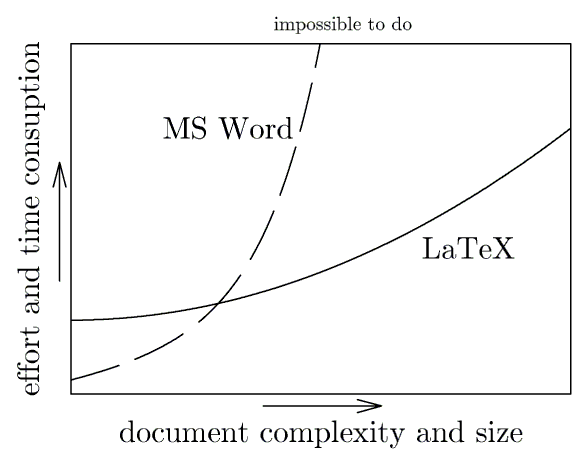
\includegraphics[width=0.4\linewidth]{word_vs_latex_curve.png}
		\caption{利用 \LaTeX\ 與 Word 處理不同複雜度的文件時,分別所需的時間與精力}
		\label{fig:LaTeX vs. Word curve}
	\end{figure}
	\pagebreak
	也正因為兩套軟體的性質迥異,許多梗圖就因此誕生...
	\begin{figure}[H]
		\centering
		\mpimg{0.4}{EXtjfNvUMAIyQ_G.jpg}
		\hspace{0.5cm}
		\mpimg{0.45}{R8ShZojm9a3L-Bq5jOFXfRzGLHa3H_r5o7-zVYLi3Wo.png}
		\caption{更多關於\LaTeX 與Word的梗圖}
	\end{figure}
	最後,既然說\LaTeX 與程式語言的運作邏輯比較相似,那就來與時下當紅的C++與Python比較吧!
	\begin{table}[H]
		\centering
		\rowcolors{2}{gray!20}{gray!10}
		\OSfamily
		\begin{tabularx}{\textwidth}{Tp{0.26\textwidth}TX|X|XT}
			\Thline
			\rowcolor{cyan!50} \diagbox[innerwidth=\linewidth, linewidth=2\arrayrulewidth]{使用軟體/屬性}{語言} &
			\thead{\LaTeX \ \ LaTeX} &
			\thead{\inlineimg{cpp_logo.png}\ \ C++} &
			\thead{\inlineimg{python-logo.png}\ \ Python} \\ \Thline
			編輯器(Editor)\ / \newline
			整合開發環境(IDE\footnotemark[2]) &
			\begin{tabitemize}
				\item {Texmaker \inlineimg{texmaker_logo.png}}
				\item {TeXstudio \inlineimg{Texstudio_Logo.png}}
				\item {TeXworks \inlineimg{TeXworks256.png}}
			\end{tabitemize} &
			\begin{tabitemize}
				\item {Dev-C++ \inlineimg{Dev_C++_logo.png}}
				\item {Code::Blocks \inlineimg{CodeBlocks_logo.png}}
			\end{tabitemize} &
			\begin{tabitemize}
				\item {PyCharm \inlineimg{PyCharm_Icon.png}}
				\item {Spyder \inlineimg{Spyder_logo.png}}
				\item {Jupyter \inlineimg{Jupyter_logo.png}}
			\end{tabitemize} \\ \hline
			編譯器(Compiler)\ / \newline
			直譯器(Interpreter) &
			\begin{tabitemize}
				\item \hologo{pdfLaTeX}
				\item \hologo{XeLaTeX}
				\item \hologo{LuaLaTeX}
			\end{tabitemize} & 
			\begin{tabitemize}
				\item {G++ \inlineimg{GNU_Compiler_Collection_logo.png}}
				\item {MSVC\footnotemark[3] \inlineimg{Visual_Studio_Icon_2019.png}}
			\end{tabitemize} &
			\begin{tabitemize}
				\item {CPython \inlineimg{cython_icon.png}}
				\item PyPy \inlineimg{pypy-logo.png}
			\end{tabitemize} \\ \hline
			輸出(Output) & .pdf \ \inlineimg{PDF_file_icon.png} & {.exe \inlineimg{windows-exe-icon-1.jpg}} & {(\ .exe \inlineimg{windows-exe-icon-1.jpg}\ )} \\ \Thline
		\end{tabularx}
		\caption{\LaTeX\ vs C++ vs Python}
		\label{tab:LaTeX vs C++ vs Python}
	\end{table}
	\footnotetext[2]{Integrated Development Environment, 整合開發環境}
	\footnotetext[3]{Microsoft Visual C++}
\end{document}